% Fixture: environments, the phases around the body, and a discarded shipout.
%
% Known answers, on pdfLaTeX, XeLaTeX and LuaLaTeX with prumo's default environments
% (tests/fixtures.rs::environments_fixture_claims, tests/tex.rs for the PDF):
%  1. tikzpicture is recorded 4 times: once in the body and 3 times inside tabularx,
%     which typesets its body once per trial width. tabularx, longtable and lstlisting
%     are recorded once each.
%  2. The inline \tikz in the text and the one in \AtBeginDocument are not environments
%     and leave no env record.
%  3. The PDF has 3 pages. 4 shipouts start: the second is discarded (a ship with no page),
%     so `ship 2` appears twice.
%  4. The longtable crosses a page break: page 2 ships inside it, and its time leaves that
%     shipout out.
%  5. \AtBeginDocument work runs between predoc and docstart; page 1 counts from docstart.
%  6. Page 3 ships after enddoc (the \AtEndDocument text is on it) and before lastpage.
%  7. The PDF is byte-identical with and without the probe.
\documentclass{article}
\usepackage{tikz}
\usepackage{tabularx}
\usepackage{longtable}
\usepackage{listings}
% Work for the begin-document phase; an inline \tikz is not an environment.
\AtBeginDocument{\sbox0{\tikz\draw (0,0) circle (1);}}
\AtEndDocument{\par Last words, typeset by \texttt{\string\AtEndDocument}.}
\newcommand\tenrows{%
  a & b\\ a & b\\ a & b\\ a & b\\ a & b\\ a & b\\ a & b\\ a & b\\ a & b\\ a & b\\}
\begin{document}
\section{Pictures}
A picture inline, \tikz\draw (0,0) -- (1,0);, is not an environment.

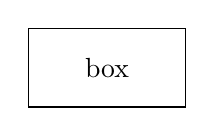
\begin{tikzpicture}
  \draw (0,0) rectangle (2,1);
  \node at (1,0.5) {box};
\end{tikzpicture}

\begin{tabularx}{\linewidth}{lX}
  a & 
\begin{tikzpicture}\draw (0,0) circle (0.2);\end{tikzpicture} \\
\end{tabularx}

\begin{lstlisting}
for i in range(3): print(i)
\end{lstlisting}
\clearpage
% A page a package throws away: shipout/before runs, shipout/after does not.
\AddToHookNext{shipout/before}{\DiscardShipoutBox}
This page is discarded.
\clearpage
\begin{longtable}{ll}
\tenrows\tenrows\tenrows\tenrows\tenrows\tenrows
\end{longtable}
\end{document}
